\documentclass{article}
\usepackage[UTF8]{ctex}
\usepackage{graphicx}
\usepackage{float}
\usepackage{hyperref}
\usepackage{amsmath}
\usepackage{amssymb}
\usepackage{booktabs}
\usepackage{multirow}
\usepackage{array}
\usepackage{geometry}
\geometry{a4paper, margin=1in}
\usepackage{unicode-math}
\setmonofont{DejaVu Sans Mono}
\usepackage{pdfpages}
\usepackage{listings}
\lstset{
    basicstyle=\ttfamily\small,
    breaklines=true,
    postbreak=\raisebox{0ex}[0ex][0ex]{\ensuremath{\hookrightarrow\space}},
    columns=fullflexible,
    frame=single,
    showstringspaces=true,
    keepspaces=true,
    tabsize=4,
    xleftmargin=2em,
    xrightmargin=2em
}

\usepackage{fancyvrb}
\usepackage{fontspec}
\setmonofont{DejaVu Sans Mono}
\setmainfont{SimSun}
\usepackage{fancyhdr}
\usepackage{lastpage}
\pagestyle{fancy}
\fancyhf{}
\fancyhead[C]{Xiamen University Malaysia}
\fancyfoot[C]{\thepage/\pageref{LastPage}}
% \fancyfoot[C]{\thepage/28}
\fancyhead[R]{\leftmark}
\fancyhead[L]{G0191 Face Recognition}


\title{基于 PCA 的人脸识别项目报告}
\date{2025 February Semester Week 5}
\author{
    Liu Zhen (AIT2409033) \\
    Cui Zeyu (DSC2409006) \\ \\
    \href{https://github.com/zeyu10/FaceRecognition}{Project Website (GitHub)}
}

\begin{document}
\maketitle

\tableofcontents
\newpage

\section{引言}
在当今数字化时代,人脸识别技术作为生物识别领域的核心技术之一,凭借其独特性、便捷性和高效性,在众多领域得到了广泛应用。从安防监控领域的实时人员身份识别,保障公共场所的安全;到门禁系统的智能化管理,提升办公场所和住宅小区的安全性;再到金融支付领域的刷脸支付,为用户带来便捷、安全的支付体验,人脸识别技术正深刻改变着人们的生活和工作方式。

本项目聚焦于设计并实现一个基于主成分分析(PCA)的人脸识别系统。其目的在于为各类场景下的人员身份识别需求提供可靠、高效的解决方案。通过收集、处理大量人脸数据,运用 PCA 技术提取关键特征,并结合先进的分类算法,该系统能够准确地识别出人员身份,为实际应用提供有力支持。
\newpage
\section{使用方法}

\subsection{环境搭建与数据准备}

\subsubsection{安装依赖库}
本系统基于 Python 语言开发,运行前需确保已安装 Python 环境。项目主要依赖 \texttt{OpenCV}、\texttt{NumPy}、\texttt{PyQt5} 等库。可使用 \texttt{pip} 工具进行安装,在命令行中依次执行 \texttt{pip install opencv-python}、\texttt{pip install numpy}、\texttt{pip install PyQt5} 等命令,完成依赖库的安装。

\subsubsection{收集人脸数据}
按照项目要求,需收集至少 100 张人脸图像,且这些图像应来自超过 20 个人。将收集到的人脸图像按照人员进行分类,分别存储在不同的文件夹下。每个文件夹的名称作为对应人员的标识,图像格式支持 \texttt{.jpg}、\texttt{.jpeg}、\texttt{.png}。确保图像质量良好,背景相对简单,以提高后续识别的准确率。

\subsection{项目内容概览}

\subsubsection{项目结构概览}
\begin{lstlisting}[basicstyle=\small\ttfamily]
FaceRecognition/
│
├── Config.py                # 配置文件,包含系统参数和常量
├── Dataset.py               # 数据集处理模块,负责数据导入、处理和保存
├── FaceDetector.py          # 人脸检测模块,负责检测和预处理人脸图像
├── Recognizer.py            # 识别模块,实现 PCA 和 kNN 算法
├── MainWindow.py            # 主界面模块,提供用户界面和系统功能集成
│
├── Caffemodel/              # 预训练的深度学习模型文件
│   ├── deploy.prototxt      # 模型配置文件
│   └── res10_300x300_ssd_iter_140000.caffemodel
│                            # 模型权重文件
│
├── Dataset/                 # 数据集文件夹,存储原始图像和预处理后的数据
│   ├── Att_Faces/           # 包含 Att_Faces 数据集的原始图像
│   ├── Dataset_Personal/    # 包含带背景的个人数据集
│   ├── Dataset_Pure/        # 包含纯个人数据集
│   ├── Dataset_Personal_Big.pkl    # 大型个人数据集的预处理文件
│   ├── Dataset_Personal_Small.pkl  # 小型个人数据集的预处理文件
│   └── Dataset_Personal_with_AttFaces.pkl
│                                   # 包含 Att_Faces 的个人数据集预处理文件
│
├── Report.pdf               # 项目报告文档
\end{lstlisting}

\subsubsection{文件功能说明}

\paragraph{1. Config.py}
\begin{itemize}
    \item \textbf{功能}:配置文件,定义了系统中使用的常量参数。
    \item \textbf{关键参数}:
    \begin{itemize}
        \item \texttt{FACE\_EXTEND\_FACTOR}:人脸区域扩展因子。
        \item \texttt{TRAIN\_RATIO}:训练集和测试集的分割比例。
        \item \texttt{KEEP\_COMPONENTS}:PCA 保留的主成分比例。
        \item \texttt{RECOGNITION\_SIZE}:人脸图像的统一尺寸。
        \item \texttt{CANDIDATE\_K}:kNN 算法中候选的 k 值列表。
    \end{itemize}
\end{itemize}

\paragraph{2. Dataset.py}
\begin{itemize}
    \item \textbf{功能}:数据集处理模块,负责数据导入、处理和保存。
    \item \textbf{核心功能}:
    \begin{itemize}
        \item \texttt{import\_dataset}:从文件夹导入人脸图像数据,并进行预处理。
        \item \texttt{save\_dataset}:将数据集保存为 \texttt{.pkl} 文件。
        \item \texttt{load\_dataset}:从 \texttt{.pkl} 文件加载数据集。
        \item \texttt{split\_dataset}:将数据集分割为训练集和测试集。
    \end{itemize}
\end{itemize}

\paragraph{3. FaceDetector.py}
\begin{itemize}
    \item \textbf{功能}:人脸检测模块,负责检测和预处理人脸图像。
    \item \textbf{核心功能}:
    \begin{itemize}
        \item \texttt{detect\_faces}:使用深度学习模型检测人脸。
        \item \texttt{get\_most\_confident\_face\_region}:获取最自信的人脸区域。
        \item \texttt{enhance\_image}:对图像进行增强和背景去除。
    \end{itemize}
\end{itemize}

\paragraph{4. Recognizer.py}
\begin{itemize}
    \item \textbf{功能}:识别模块,实现 PCA 和 kNN 算法。
    \item \textbf{核心功能}:
    \begin{itemize}
        \item \texttt{fit}:使用 PCA 进行特征提取。
        \item \texttt{evaluate}:评估模型的准确率。
        \item \texttt{predict}:使用 kNN 算法进行人脸识别。
        \item \texttt{kNNR\_classifier}:kNN 分类器实现。
    \end{itemize}
\end{itemize}

\paragraph{5. MainWindow.py}
\begin{itemize}
    \item \textbf{功能}:主界面模块,提供用户界面和系统功能集成。
    \item \textbf{核心功能}:
    \begin{itemize}
        \item \texttt{MainWindow}:主窗口类,集成数据导入、模型训练、相机操作等功能。
        \item \texttt{CameraWindows}:相机窗口类,提供实时人脸检测和识别功能。
        \item \texttt{slot\_add\_face}:在界面中添加人脸数据。
        \item \texttt{on\_train\_model}:训练模型并显示训练进度。
    \end{itemize}
\end{itemize}

\paragraph{6. Caffemodel/}
\begin{itemize}
    \item \textbf{功能}:存放预训练的深度学习模型文件。
    \item \textbf{文件}:
    \begin{itemize}
        \item \texttt{deploy.prototxt}:模型配置文件。
        \item \texttt{res10\_300x300\_ssd\_iter\_140000.caffemodel}:模型权重文件。
    \end{itemize}
\end{itemize}

\paragraph{7. Dataset/}
\begin{itemize}
    \item \textbf{功能}:存储数据集的原始图像、储存数据集的预处理文件。
    \item \textbf{内容}:
    \begin{itemize}
        \item \texttt{Att\_Faces/}:存储 Att\_Faces 数据集的原始图像,共 \textbf{400} 张。
        \item \texttt{Dataset\_Personal\_With\_Background/}:存储带背景的小组成员数据集,共 \textbf{65} 张。
        \item \texttt{Dataset\_Pure/}:存储纯个人数据集,共 \textbf{103} 张。
        \item \texttt{Dataset\_Personal\_Big.pkl}:存储大型个人数据集的预处理文件
        \begin{itemize}
            \item 包含 \texttt{Dataset\_Personal\_With\_Background/} + \texttt{Dataset\_Pure/} 数据集。
        \end{itemize}
            \item \texttt{Dataset\_Personal\_Small.pkl}:存储小型个人数据集的预处理文件
        \begin{itemize}
            \item 仅有 \texttt{Dataset\_Personal\_With\_Background/} 数据集。
        \end{itemize}
        \item \texttt{Dataset\_Personal\_with\_Attfaces.pkl}:存储全部的个人数据集预处理文件
        \begin{itemize}
            \item 包含 \texttt{Dataset\_Personal\_With\_Background/} + \texttt{Dataset\_Pure/} + \texttt{Att\_Faces/} 全部数据集。
        \end{itemize}
    \end{itemize}
\end{itemize}

\subsection{项目操作流程}

\subsubsection{启动项目}
找到项目目录中的 \texttt{MainWindow.py} 文件,在命令行中运行 \texttt{python MainWindow.py} 命令,启动人脸识别系统。系统启动后,会弹出主窗口,该窗口集成了数据导入、模型训练、相机操作、数据集管理等功能按钮,以及图像显示区域和数据表格。

\begin{figure}[H]
    \centering
    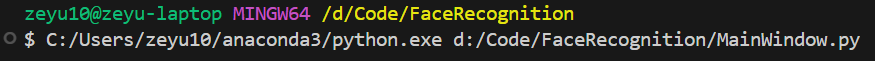
\includegraphics[width=0.8\textwidth]{Img/PixPin_2025-03-09_00-37-52.png}
    \caption{命令行启动项目主窗口}
\end{figure}

\subsubsection{导入数据}
\begin{itemize}
    \item 点击主窗口中的 \texttt{Import From Folder} 按钮,系统会弹出文件选择对话框。在对话框中导航至存储人脸图像的文件夹,选中该文件夹后点击“确定”。
    \item 此时系统会弹出询问框,询问是否去除人脸背景。若选择“是”,系统将在后续处理中运用图像处理技术去除人脸背景;若选择“否”,则保留原始图像背景。
    \item 系统开始读取所选文件夹及其子文件夹中的图像文件。对于尺寸过大(像素超过 62500)的图像,系统会基于 \texttt{OpenCV} 的 \texttt{dnn} 模块进行人脸检测,获取最自信的人脸区域,并依据配置文件中的 \texttt{FACE\_EXTEND\_FACTOR} 参数进行扩展裁剪。随后,将图像统一调整为尺寸为 \texttt{RECOGNITION\_SIZE}(100x100)的图像。
    \item 处理完成的图像数据会存储在系统的数据集内。同时,在主窗口的数据表格中,会显示每张图像对应的 ID、姓名(根据文件夹名确定)、路径以及是否添加到模型的勾选框等信息。
\end{itemize}

\begin{figure}[H]
    \centering
    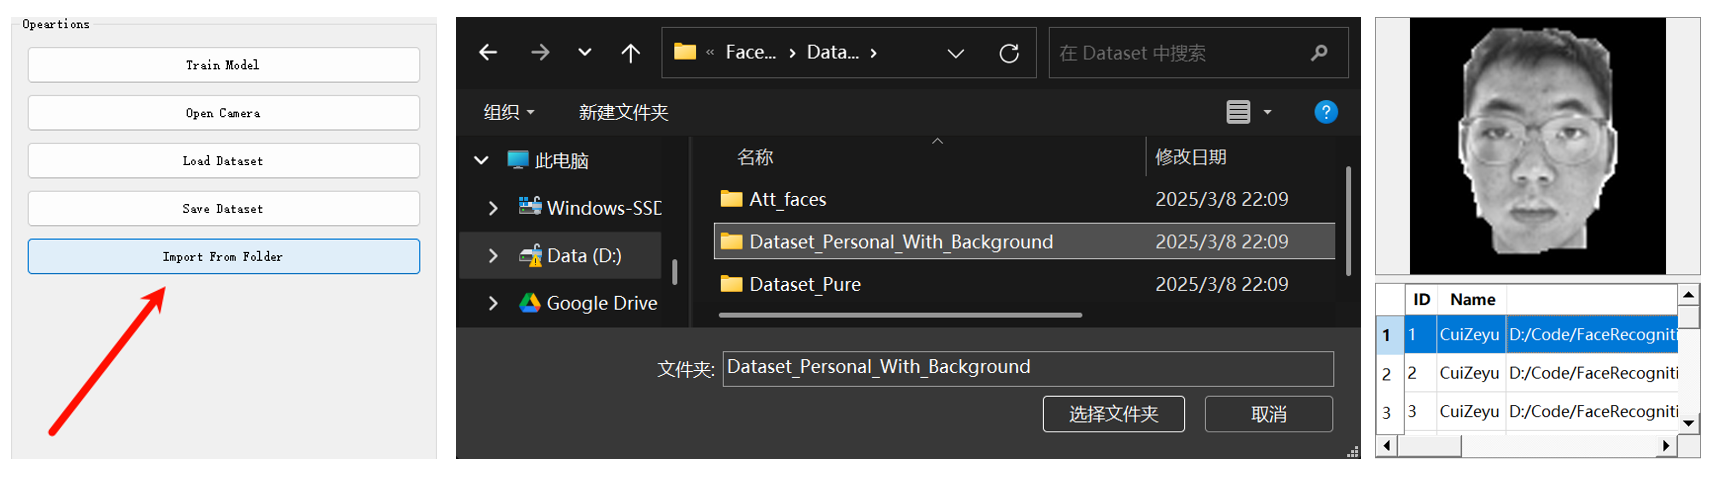
\includegraphics[width=0.8\textwidth]{Img/PixPin_2025-03-09_00-48-16.png}
    \caption{导入数据界面}
\end{figure}

\subsubsection{模型训练}
\begin{itemize}
    \item 在进行模型训练前,需确保数据表格中已导入足够的人脸数据。若数据集为空,点击 \texttt{Train Model} 按钮时,系统会弹出错误提示框,提示用户先导入数据。
    \item 确认数据无误后,点击 \texttt{Train Model} 按钮,系统开始模型训练。训练过程中,主窗口底部的进度条会实时显示训练的进展情况。
    \item 模型训练包含多个关键步骤,首先对导入的数据进行处理,提取关键特征;接着计算如均值脸、协方差矩阵、特征值和特征向量等相关参数;最后对模型进行评估,确定模型的性能指标。
    \item 训练完成后,主窗口的状态栏会显示训练所花费的时间以及模型的准确率,方便用户了解模型训练效果。
    \item 可在主窗口中导入多个文件夹进行训练与识别。
\end{itemize}

\begin{figure}[H]
    \centering
    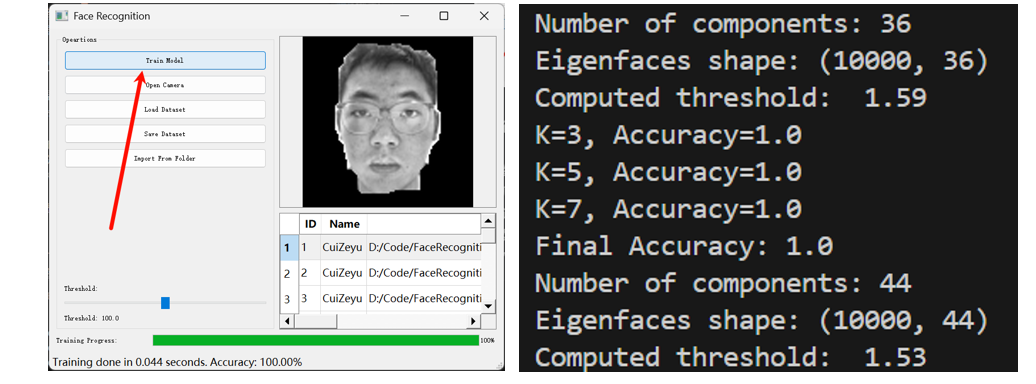
\includegraphics[width=0.8\textwidth]{Img/PixPin_2025-03-09_00-52-21.png}
    \caption{模型训练界面}
\end{figure}

\subsubsection{开启相机进行识别}
\begin{itemize}
    \item 在主窗口中点击 \texttt{Open Camera} 按钮。若首次打开相机,系统会弹出相机选择窗口,列出当前设备上可用的相机设备。用户可根据实际情况选择对应的相机设备(若只有一个相机设备,系统会自动选择并打开)。相机窗口打开后,用户可实时查看相机拍摄的画面。
    \item 在相机窗口中,点击 \texttt{Recognize Face} 按钮。若模型已成功训练完成,该按钮会变为 \texttt{Stop Recognizing},同时开启人脸识别功能。系统会在相机实时画面中检测人脸,一旦检测到人脸,会对其进行一系列处理和识别操作。
    \item 识别结果会实时显示在相机画面上。若识别出是已知人员,会在画面上显示人员姓名;若未识别出,则显示 \texttt{Stranger}。此外,在相机窗口的右侧小窗口中,会分别显示检测到的人脸图像以及预测的匹配图像(若识别成功),方便用户直观对比。
    \item 在相机窗口中,用户可通过勾选 \texttt{Remove Background} 复选框来决定是否对检测到的人脸图像进行背景去除处理。勾选后,系统会在处理人脸图像时运用相关图像处理算法去除背景,以进一步提高识别效果。
    \item 点击相机窗口中的 \texttt{Screenshot} 按钮,可对当前相机画面进行拍照操作。拍摄的照片会以 \texttt{Screenshot\_yy\_dd\_hh\_mm\_ss.jpg} 的格式保存在程序运行目录下,同时相机窗口的状态栏会提示照片保存的文件名,方便用户查找。
\end{itemize}

\begin{figure}[H]
    \centering
    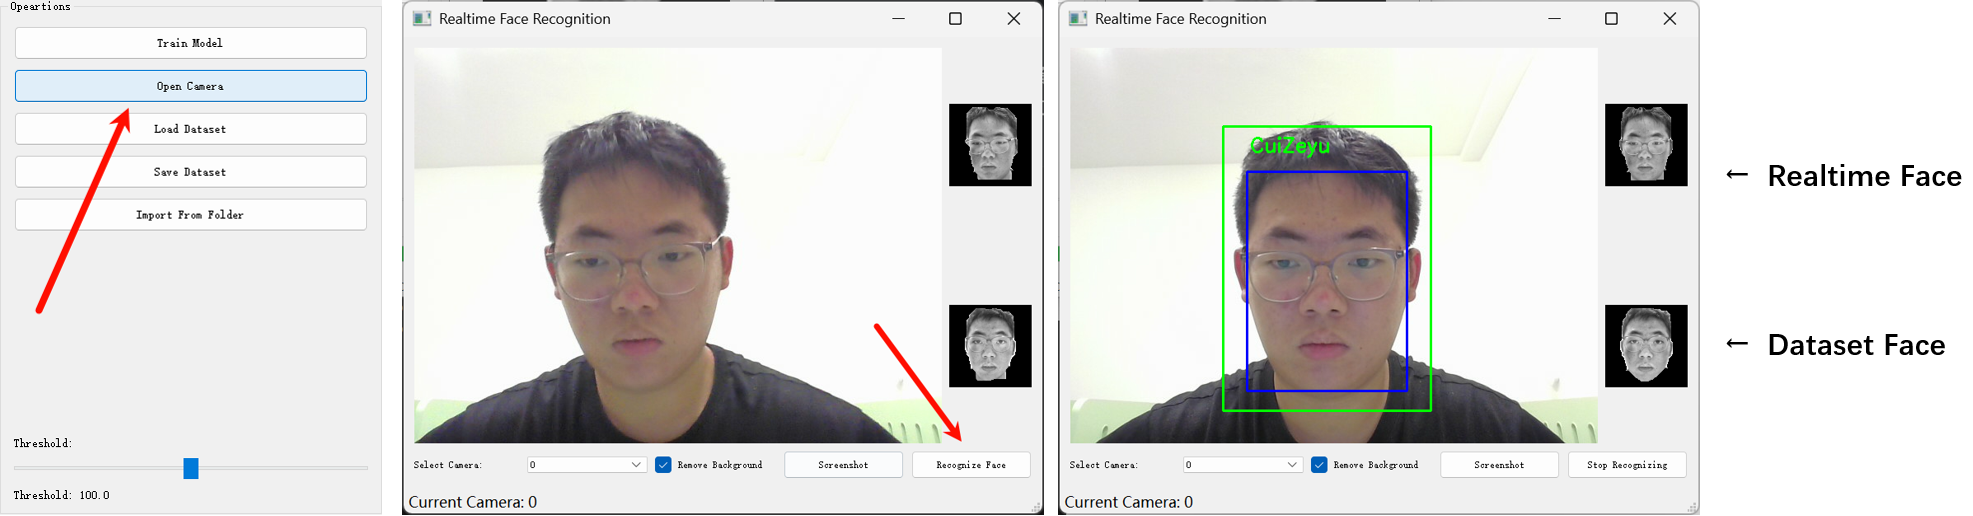
\includegraphics[width=0.8\textwidth]{Img/PixPin_2025-03-09_00-59-57.png}
    \caption{调用摄像头测试 (Camera 0)}
\end{figure}

\begin{figure}[H]
    \centering
    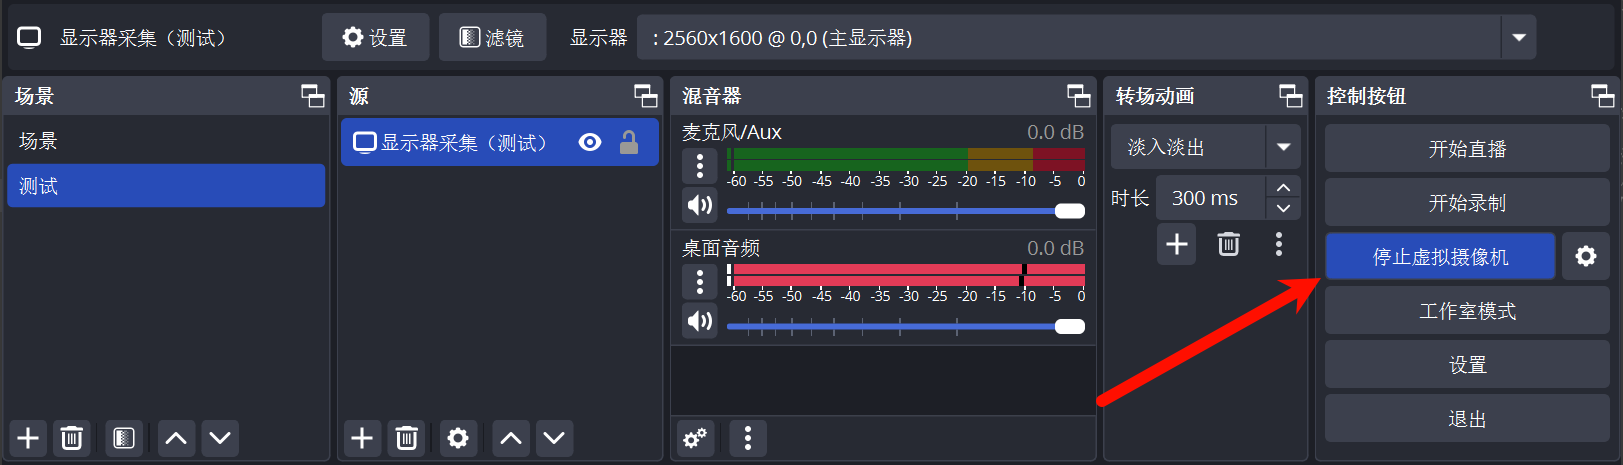
\includegraphics[width=0.8\textwidth]{Img/PixPin_2025-03-09_10-58-44.png}
    \caption{本地数据集测试 (Camera 1 or Camera 2,需借助 OBS 虚拟摄像头)}
\end{figure}

\begin{figure}[H]
    \centering
    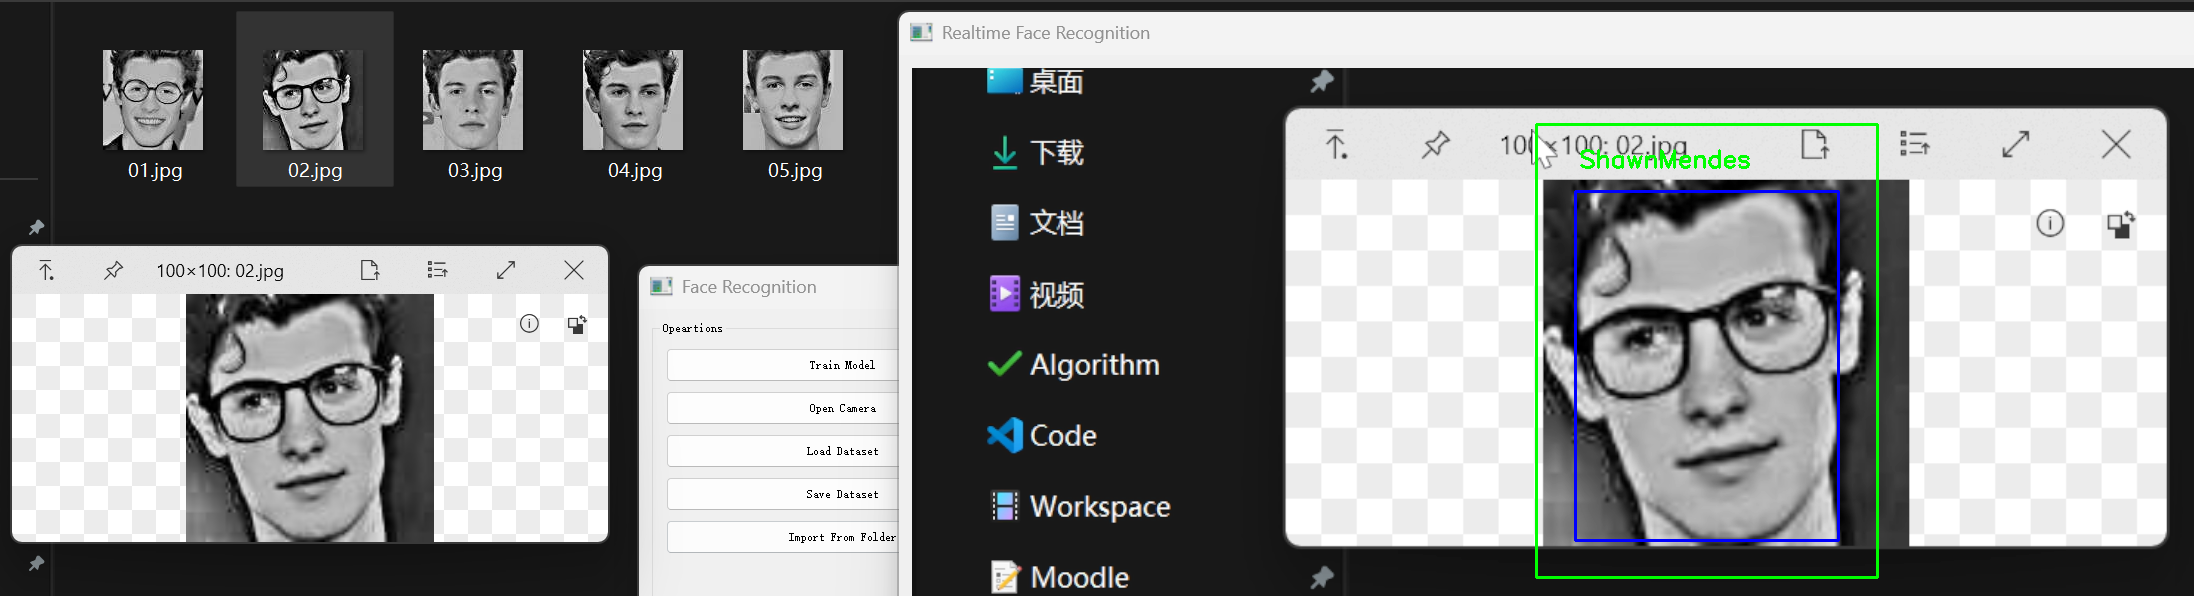
\includegraphics[width=0.8\textwidth]{Img/PixPin_2025-03-09_11-11-17.png}
    \caption{本地数据集测试}
\end{figure}

\subsubsection{调整识别阈值}
\begin{itemize}
    \item 在主窗口的左侧操作面板中,用户可以看到一个滑块控件,用于调整人脸识别的阈值。阈值决定了系统在识别过程中对相似度的要求。阈值越低,系统对相似度的要求越宽松,识别结果可能包含更多的误识别;阈值越高,系统对相似度的要求越严格,识别结果更加准确,但可能会漏掉一些相似度较低的正确识别。
    \item 用户可以通过拖动滑块来调整阈值,滑块的值范围从 0 到 200,对应的阈值范围为 0.0 到 2.0。系统默认的初始值为 100,对应的阈值为 1.0。用户可以根据实际需求调整阈值,以达到最佳的识别效果。
    \item 调整阈值后,系统会实时更新识别结果,用户可以通过观察相机窗口中的识别结果来判断当前阈值是否合适。
\end{itemize}

\begin{figure}[H]
    \centering
    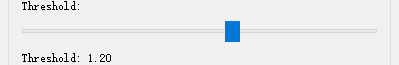
\includegraphics[width=0.6\textwidth]{Img/PixPin_2025-03-09_01-02-00.png}
    \caption{调整识别阈值界面}
\end{figure}

\subsubsection{数据集操作}
\begin{itemize}
    \item 点击主窗口中的 \texttt{Save Dataset} 按钮,系统会弹出文件保存对话框。用户可在对话框中选择保存路径,并输入文件名(文件格式为 \texttt{.pkl}),点击 \texttt{保存} 后,系统会将当前系统中的数据集保存下来,以便后续使用。
\end{itemize}

\begin{figure}[H]
    \centering
    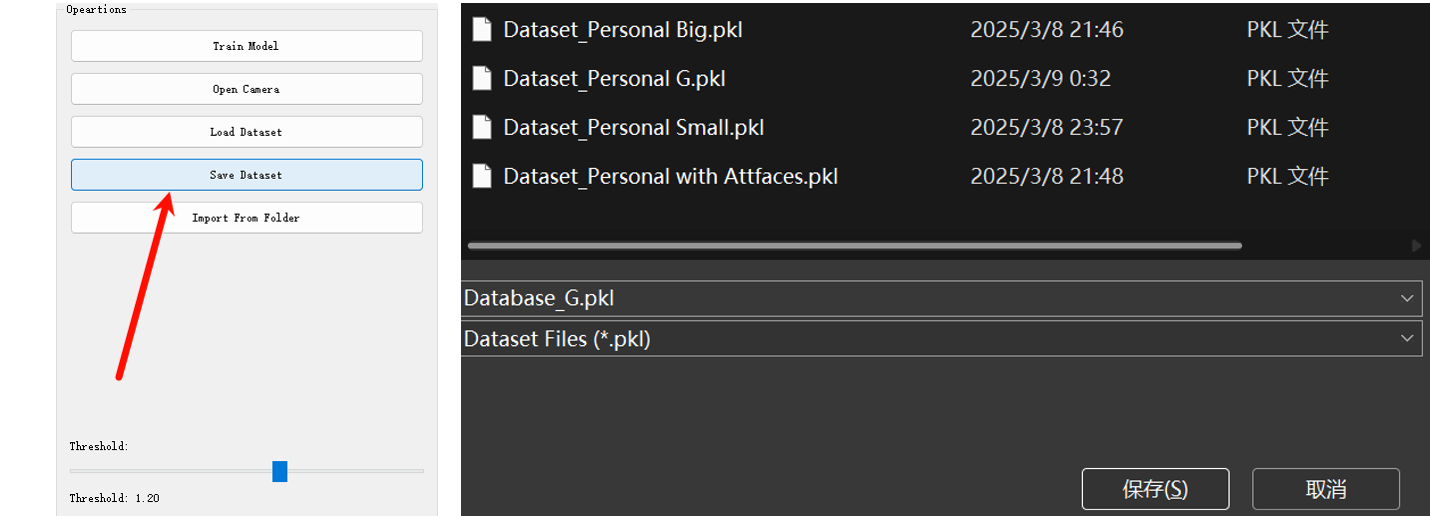
\includegraphics[width=0.8\textwidth]{Img/PixPin_2025-03-09_01-05-24.png}
    \caption{保存数据集界面}
\end{figure}

\begin{itemize}
    \item 点击 \texttt{Load Dataset} 按钮,系统弹出文件选择对话框。选择之前保存的数据集文件(\texttt{.pkl}),系统会加载数据集,并将数据显示在主窗口的数据表格中,同时更新相关数据索引,方便用户继续进行后续操作。
\end{itemize}

\begin{figure}[H]
    \centering
    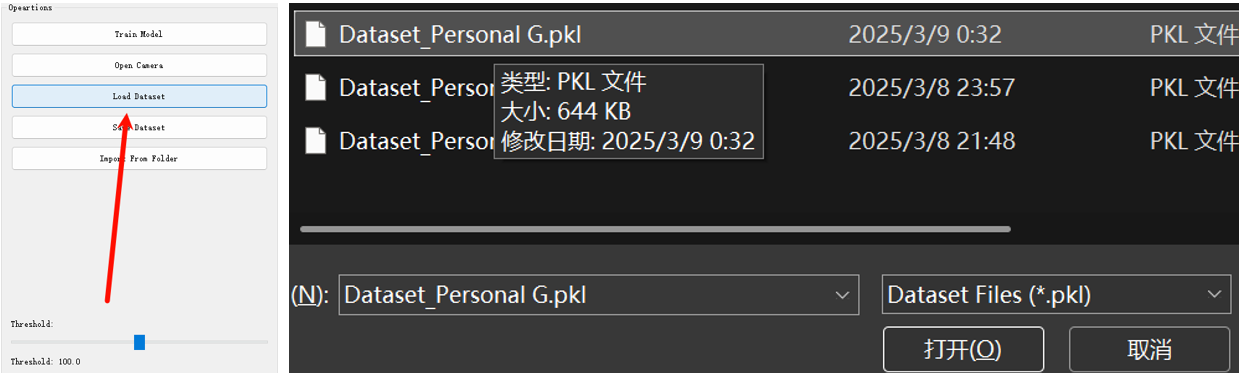
\includegraphics[width=0.8\textwidth]{Img/PixPin_2025-03-09_02-37-48.png}
    \caption{加载数据集界面}
\end{figure}
\newpage
\section{重要原理}

\subsection{主成分分析(PCA)}

\subsubsection{PCA 基本原理}
PCA 是一种强大的数据降维技术,其核心目标是通过线性变换,将高维数据投影到一组正交的主成分上,使得数据在低维空间中能够保留大部分的方差信息。在人脸识别领域,每一张人脸图像都可以看作是一个高维向量,这些向量构成了一个高维的数据空间。通过 PCA,我们能够找到那些能够最大程度解释数据方差的方向,这些方向对应的向量就是所谓的“特征脸”。利用这些特征脸,我们可以将高维的人脸图像数据投影到一个低维空间中,实现数据降维的同时,保留关键的识别特征,从而大大减少计算量和存储需求。

\subsubsection{PCA 数学原理}

\paragraph{数据矩阵构建}
假设有 $m$ 个人脸图像,每个图像被表示为一个 $n$ 维向量(假设图像已被拉直成一维向量),则可以构建一个大小为 $n\times m$ 的数据矩阵 $X$,其中每一列代表一个人脸图像向量。

\paragraph{计算均值向量}
计算数据矩阵 $X$ 的均值向量 $\mu$,公式为:
\[
\mu=\frac{1}{m}\sum_{i = 1}^{m}x_{i}
\]
其中,$x_{i}$ 表示第 $i$ 个图像向量。均值向量 $\mu$ 代表了数据的中心趋势。从几何角度来看,它是所有数据点在 $n$ 维空间中的重心。在人脸识别中,均值脸可以看作是所有人脸的平均模样,反映了人脸的基本特征。

\begin{figure}[H]
    \centering
    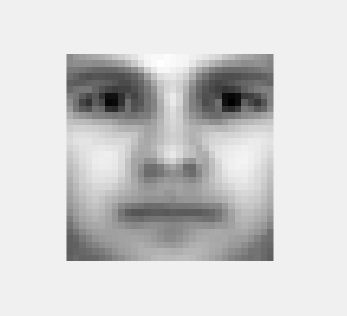
\includegraphics[width=0.5\textwidth]{Img/v2-918060b552a96c398d46f84574d5f2e4_1440w.png}
    \caption{“平均脸”,即所有人脸的平均}
\end{figure}

\paragraph{数据中心化}
将数据矩阵 $X$ 中的每个向量减去均值向量 $\mu$,得到中心化的数据矩阵 $X_{centered}$,即:
\[
X_{centered}=X - \mu\mathbf{1}^{T}
\]
其中,$\mathbf{1}$ 是一个大小为 $m$ 的全 1 向量。数据中心化的目的是使数据分布以原点为中心,消除数据的平移影响,突出数据的差异特征,为后续的特征提取做准备。经过中心化后,数据的均值变为零,使得后续计算协方差矩阵时更加方便和准确。

\begin{figure}[H]
    \centering
    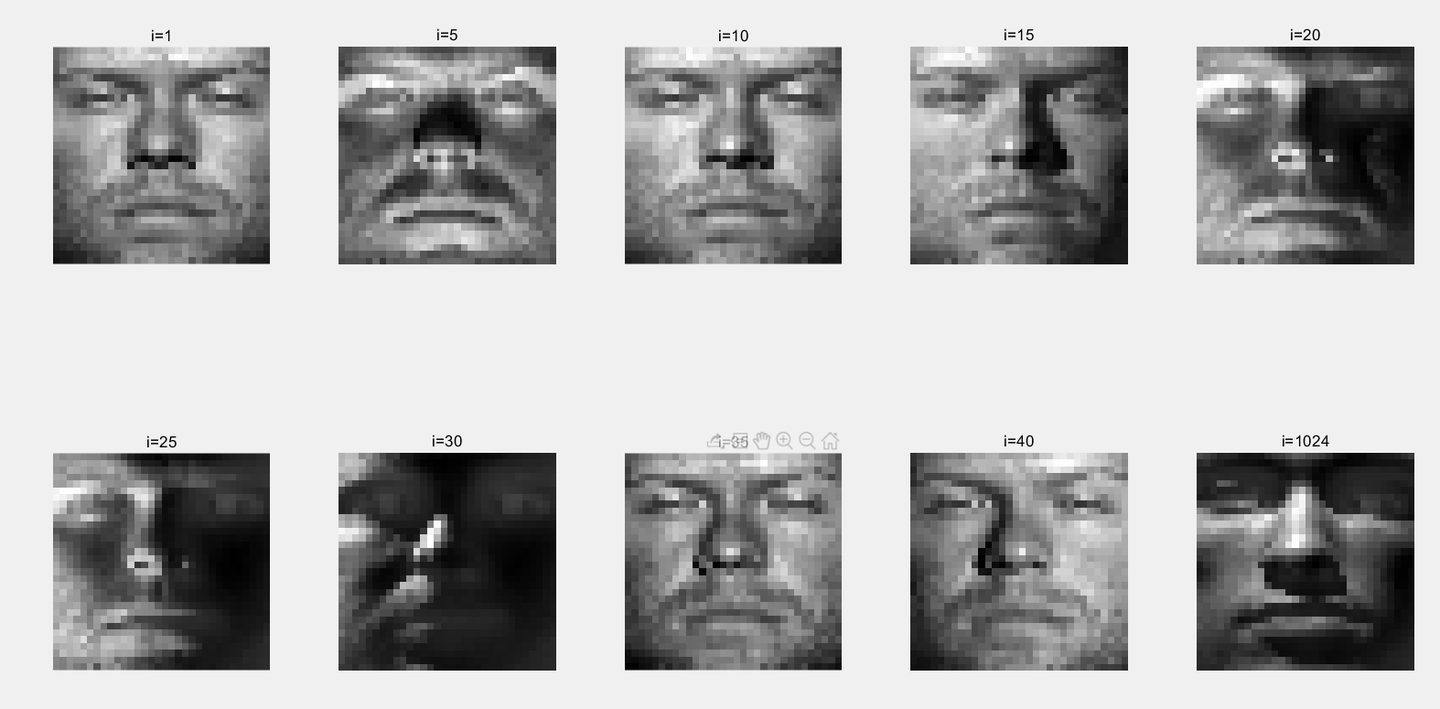
\includegraphics[width=0.8\textwidth]{Img/v2-65a459d10dbf796dcd4dbfec736c810a_1440w.png}
    \caption{原始数据在减去平均脸后得到的中心化的数据}
\end{figure}

\paragraph{计算协方差矩阵}
计算中心化后数据矩阵 $X_{centered}$ 的协方差矩阵 $C$,公式为:
\[
C=\frac{1}{m - 1}X_{centered}X_{centered}^{T}
\]
协方差矩阵 $C$ 反映了数据各个维度之间的相关性,其对角线元素表示各个维度的方差,非对角线元素表示不同维度之间的协方差。在人脸识别中,协方差矩阵描述了人脸图像各个像素之间的相关性。例如,如果两个像素在不同人脸图像中的变化趋势相似,那么它们之间的协方差就会较大;反之,如果变化趋势相互独立,协方差就会接近零。

\paragraph{求解特征值和特征向量}
对协方差矩阵 $C$ 进行特征分解,求解其特征值 $\lambda_{i}$ 和特征向量 $v_{i}$,满足:
\[
Cv_{i}=\lambda_{i}v_{i}
\]
特征值 $\lambda_{i}$ 表示对应特征向量 $v_{i}$ 方向上的数据方差大小,特征向量 $v_{i}$ 则表示数据在该方向上的变化方向。从线性代数的角度来看,特征向量是协方差矩阵 $C$ 所定义的线性变换下的不变方向,而特征值则是该方向上的缩放因子。在人脸识别中,特征向量(即特征脸)代表了人脸图像中最具变化性的方向,特征值越大,说明该特征脸包含的信息越多,对数据的解释能力越强。

\begin{figure}[H]
    \centering
    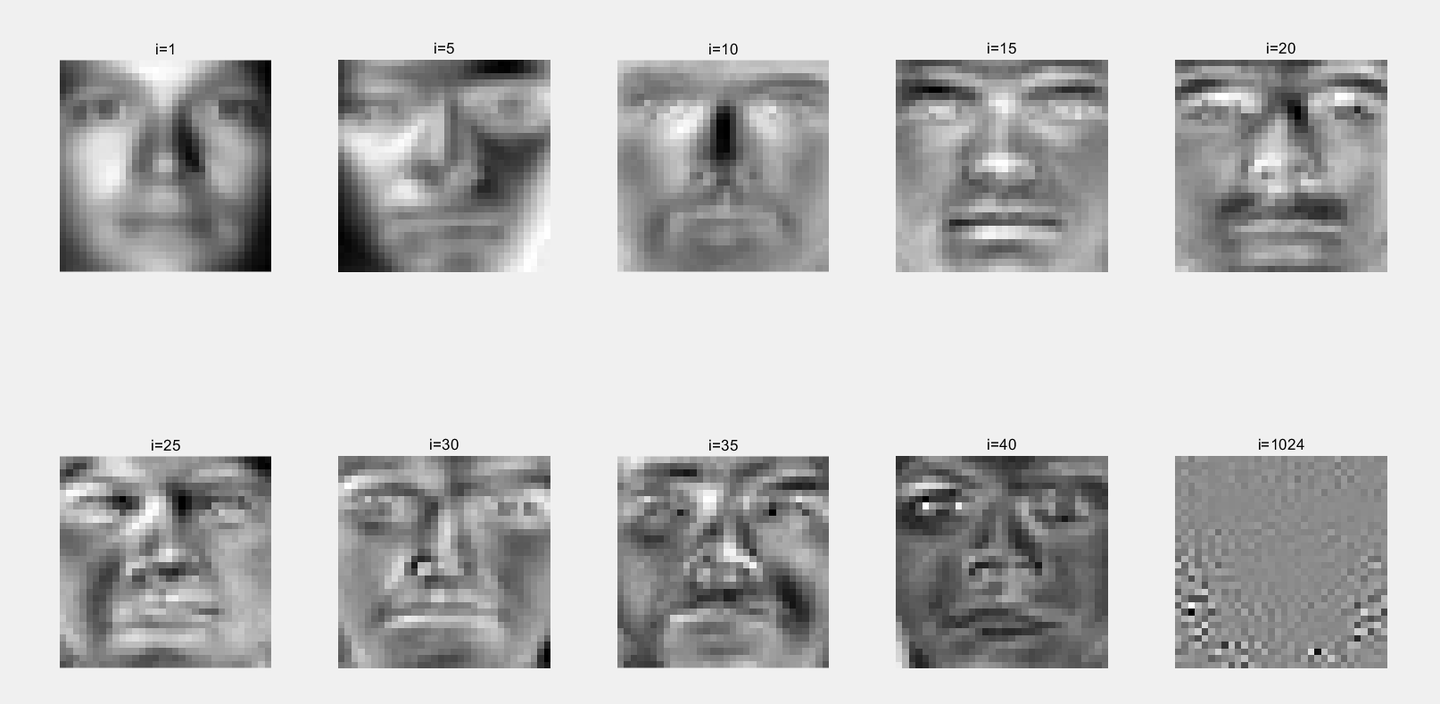
\includegraphics[width=0.8\textwidth]{Img/v2-62f392d4e1056457c15ccb4dd81dc539_1440w.png}
    \caption{把特征脸按照特征值大小排列,可以看到特征值大的脸包含的有效信息更多}
\end{figure}

\paragraph{特征值分解的理论基础}
根据线性代数中的谱定理,对于实对称矩阵(协方差矩阵 $C$ 是实对称矩阵),存在一个正交矩阵 $Q$,使得 $C = Q\Lambda Q^{T}$,其中 $\Lambda$ 是一个对角矩阵,其对角元素为 $C$ 的特征值 $\lambda_{i}$,$Q$ 的列向量为对应的特征向量 $v_{i}$。这一理论保证了我们可以通过特征分解将协方差矩阵 $C$ 对角化,从而找到数据的主成分。

\paragraph{选择主成分}
将特征值按照从大到小的顺序进行排序,即 $\lambda_{1}\geq\lambda_{2}\geq\cdots\geq\lambda_{n}$。根据设定的主成分保留比例(如 \texttt{KEEP\_COMPONENTS} 为 0.95),选择前 $k$个 特征向量作为主成分,使得累计贡献率达到设定比例。累计贡献率的计算公式为:
\[
\sum_{i = 1}^{k}\lambda_{i}/\sum_{i = 1}^{n}\lambda_{i}\geq0.95
\]
这 $k$ 个特征向量构成了特征脸空间的基向量,用于后续的数据投影和特征提取。选择合适的主成分数量是 PCA 的关键步骤之一,它需要在保留足够信息和降低数据维度之间进行权衡。如果保留的主成分过多,虽然可以保留更多的信息,但降维效果不明显;如果保留的主成分过少,则可能会丢失重要的识别特征,导致识别准确率下降。

\paragraph{数据投影}
将原始的人脸图像向量 $x$ 投影到由所选特征向量构成的低维空间中,得到投影后的向量 $y$,投影公式为:
\[
y = V^{T}(x - \mu)
\]
其中,$V$ 是由前 $k$ 个特征向量组成的矩阵,每一列是一个特征向量。通过投影,将高维的人脸图像数据转换为低维的特征向量表示,实现了数据降维。在低维空间中,数据的计算量和存储需求大大减少,同时由于保留了主要的方差信息,仍然能够进行有效的人脸识别。

\subsubsection{PCA 简单数据示例}

\begin{figure}[H]
    \centering
    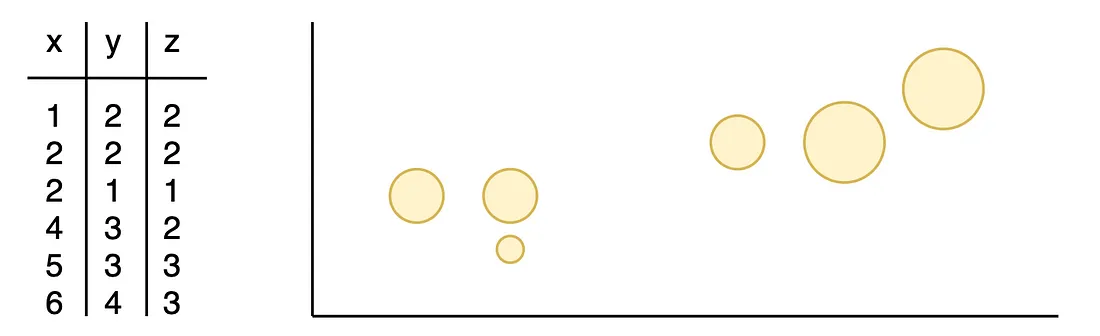
\includegraphics[width=0.7\textwidth]{Img/1_MJlSXELJ6-zNJibG5CtqIg.png}
    \caption{Plot data}
\end{figure}

\begin{figure}[H]
    \centering
    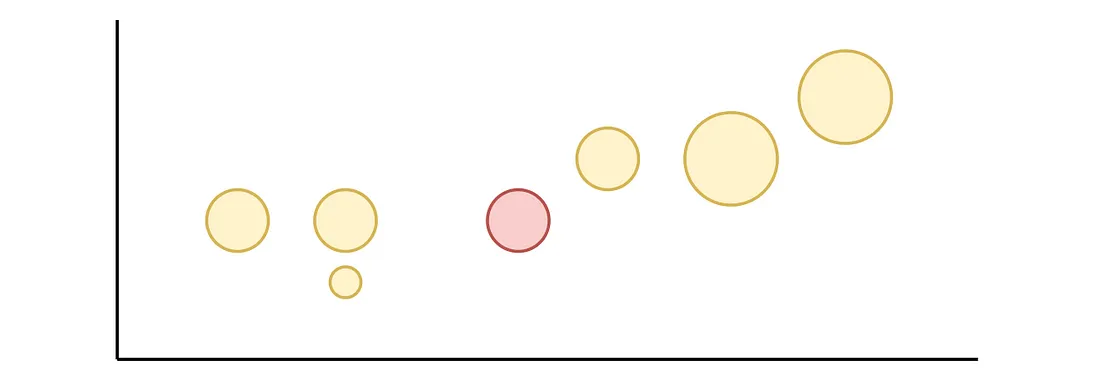
\includegraphics[width=0.7\textwidth]{Img/1_1BiMkGksH0JBOEOlf1tBTg.png}
    \caption{Find the centre of the data}
\end{figure}

\begin{figure}[H]
    \centering
    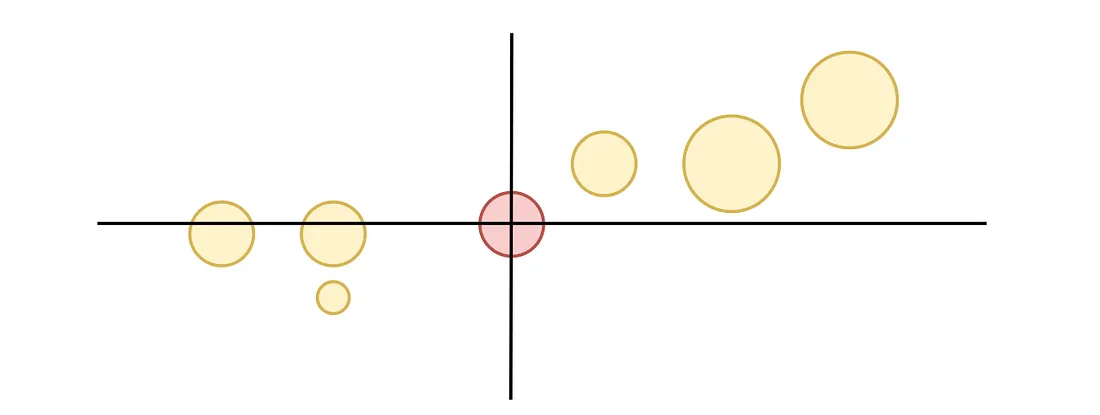
\includegraphics[width=0.7\textwidth]{Img/1_m3gnAUA9dBFQlbgWAziu3A.png}
    \caption{Shift the data points so the centre is now at (0, 0)}
\end{figure}

\begin{figure}[H]
    \centering
    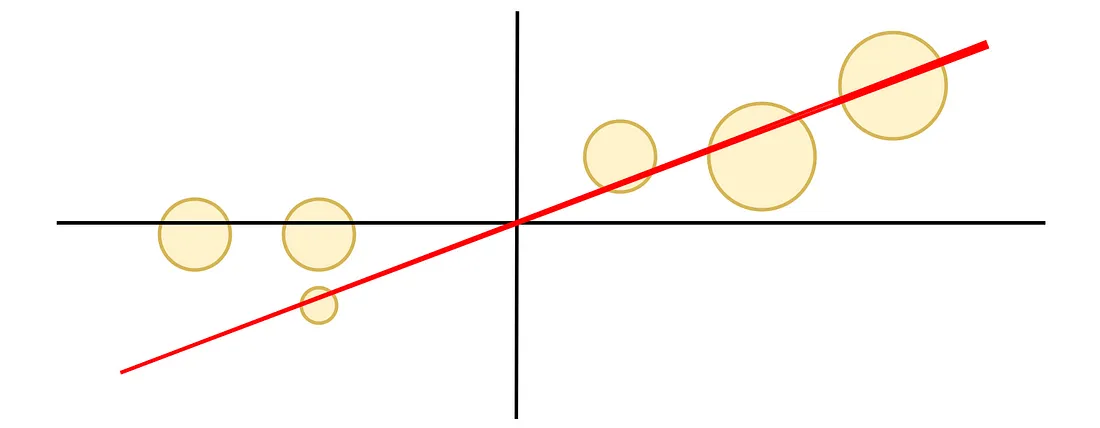
\includegraphics[width=0.7\textwidth]{Img/1_OjfIsQ5mxzfWoh3wtoBDBA.png}
    \caption{Find the line of best fit PC1}
\end{figure}

\begin{figure}[H]
    \centering
    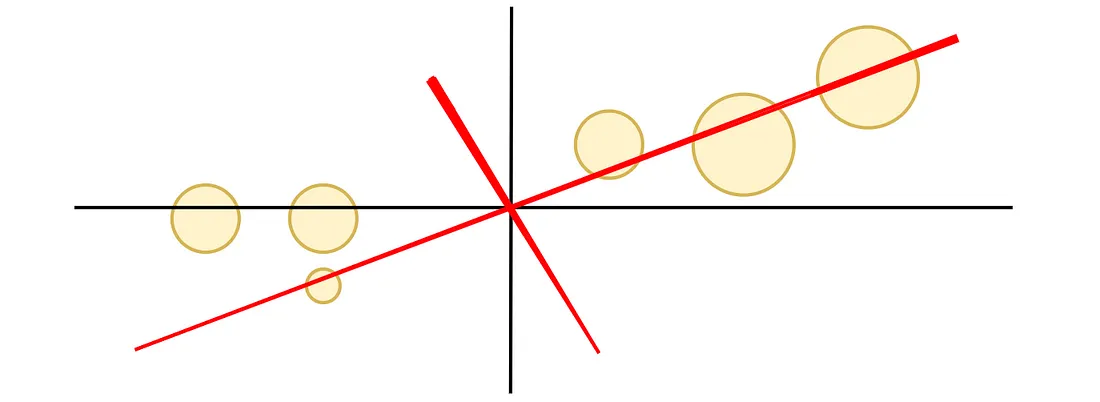
\includegraphics[width=0.7\textwidth]{Img/1_oRj5G874ukOev-uLrsq7LQ.png}
    \caption{Find another line PC2}
\end{figure}

\begin{figure}[H]
    \centering
    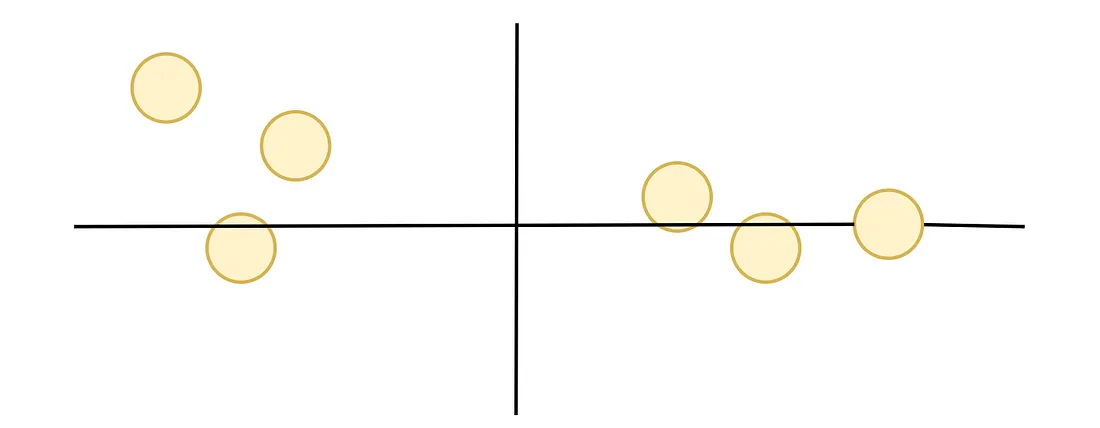
\includegraphics[width=0.7\textwidth]{Img/1_juLo2GtiuLdHhJOaNljyqw.png}
    \caption{Rotate the chart so PC1 is the x-axis and PC2 is the y-axis}
\end{figure}

\subsubsection{PCA 中高效计算特征向量的方法}
在实际应用中,直接计算高维图像的协方差矩阵的特征向量在计算量上是不可行的。例如,对于一个 $100 \times 100$ 的灰度图像,每个图像是一个 $10,000$ 维空间中的一个点,协方差矩阵 $S$ 的大小为 $10,000 \times 10,000$,具有 $10^8$ 个元素。然而,协方差矩阵的秩受到训练图像数量的限制:如果有 $N$ 个训练样本,则最多有 $N - 1$ 个对应非零特征值的特征向量。如果训练样本的数量比图像的维数低,可以通过以下方法简化特征向量的计算。

\paragraph{A. 数据矩阵的构建与预处理}
设 \( T \) 是预处理图像的矩阵,每一列对应一个减去均值图像之后的图像。假设我们有 \( N \) 个训练样本,每个样本是一个 \( D \) 维向量(例如,100×100的图像拉直成10,000维向量),则数据矩阵 \( T \) 的大小为 \( D \times N \)。

\paragraph{B. 协方差矩阵的计算}
协方差矩阵 \( S \) 可以表示为:
\[
S = \frac{1}{N-1} TT^T
\]
其中,\( TT^T \) 是一个 \( D \times D \) 的矩阵。直接计算这个矩阵的特征向量在计算量上是不可行的,特别是当 \( D \) 很大时。

\paragraph{C. 特征值分解的简化}
为了简化计算,我们可以转而计算 \( T^T T \) 的特征向量。设 \( T^T T \) 的特征向量为 \( u_i \),对应的特征值为 \( \lambda_i \),则有:
\[
T^T T u_i = \lambda_i u_i
\]
如果在等式两边乘以 \( T \),可以得到:
\[
TT^T T u_i = \lambda_i T u_i
\]
这意味着,如果 \( u_i \) 是 \( T^T T \) 的一个特征向量,则 \( v_i = T u_i \) 是 \( S \) 的一个特征向量。由于 \( T^T T \) 是一个 \( N \times N \) 的矩阵,通常 \( N \) 远小于 \( D \),因此计算 \( T^T T \) 的特征向量要容易得多。

\paragraph{D. 特征向量的归一化}
需要注意的是,通过上述方法计算得到的特征向量 \( v_i \) 没有进行归一化。为了确保特征向量的单位长度,我们需要对 \( v_i \) 进行归一化处理:
\[
v_i = \frac{T u_i}{\|T u_i\|}
\]
其中,\( \|T u_i\| \) 表示向量 \( T u_i \) 的范数。

\paragraph{E. 计算复杂度分析}
通过上述方法,我们将计算复杂度从 \( O(D^3) \) 降低到 \( O(N^3) \),其中 \( D \) 是图像的维数,\( N \) 是训练样本的数量。由于 \( N \) 通常远小于 \( D \),这种方法大大减少了计算量,使得在高维数据上进行PCA变得可行。

假设我们有 300 张 $100 \times 100$ 像素的图像,每张图像拉直后是一个 $10,000$ 维的向量。直接计算 $10,000 \times 10,000$ 的协方差矩阵的特征向量在计算上是不可行的。通过上述方法,我们只需要计算 $300 \times 300$ 的矩阵 $T^T T$ 的特征向量,然后通过简单的矩阵乘法得到协方差矩阵的特征向量。

\subsubsection{PCA 在人脸识别中的优势}
\begin{itemize}
    \item \textbf{去除冗余信息}:人脸图像数据通常存在大量的冗余信息,例如相邻像素之间的相关性较高。PCA 通过找到数据的主成分,能够去除这些冗余信息,只保留最具代表性的特征,从而提高识别效率和准确性。
    \item \textbf{降低维度灾难}:在高维空间中,数据的分布往往比较稀疏,容易导致“维度灾难”问题,即分类器的性能随着维度的增加而下降。PCA 将高维的人脸图像数据投影到低维空间中,有效缓解了维度灾难问题,使得分类器能够更好地学习和识别数据。
    \item \textbf{特征提取能力强}:PCA 提取的特征脸是数据中最具变化性的方向,它们能够捕捉到人脸的主要特征,如面部轮廓、眼睛、鼻子、嘴巴等的形状和位置信息。这些特征对于人脸识别具有重要的意义,能够提高识别的准确性。
\end{itemize}

\subsection{K 近邻重分类器(kNNR)}

\subsubsection{kNNR 基本原理}
kNNR 是一种基于实例的分类算法,在人脸识别系统中发挥着关键的分类作用。其核心思想是在训练集中寻找与待识别样本距离最近的 $k$ 个邻居,根据这 $k$ 个邻居的类别分布来预测待识别样本的类别。在本系统中,通过计算待识别图像与训练集中所有图像的距离,选取距离最近的 $k$ 个样本,然后统计这 $k$ 个样本中出现次数最多的类别作为预测结果。若存在多个类别出现次数相同的情况,则选择距离最近的样本类别作为最终预测结果。

\subsubsection{kNNR 数学原理}

\paragraph{距离度量}
假设训练集包含 $N$ 个样本,每个样本 $x_{i}$ 都有对应的类别标签 $y_{i}$。对于待识别样本 $x$,计算它与训练集中每个样本 $x_{i}$ 的距离 $d(x, x_{i})$,通常使用欧氏距离作为度量,公式为:
\[
d(x, x_{i})=\sqrt{\sum_{j = 1}^{n}(x_{j}-x_{ij})^{2}}
\]
其中,$x_{j}$ 和 $x_{ij}$ 分别是待识别样本 $x$ 和训练样本 $x_{i}$ 的第 $j$ 个特征值。欧氏距离是最常用的距离度量方法,它直观地反映了两个样本在特征空间中的几何距离。在人脸识别中,欧氏距离可以衡量两个人脸图像在特征空间中的相似度,距离越小,说明两个图像越相似。
\begin{figure}[H]
    \centering
    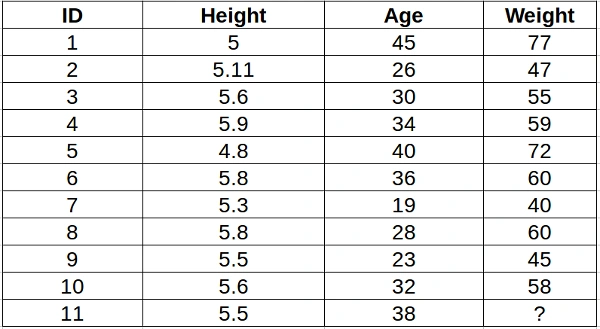
\includegraphics[width=0.7\textwidth]{Img/Screenshot-from-2018-08-22-15-03-42.png}
    \caption{Simple example table}
\end{figure}

\begin{figure}[H]
    \centering
    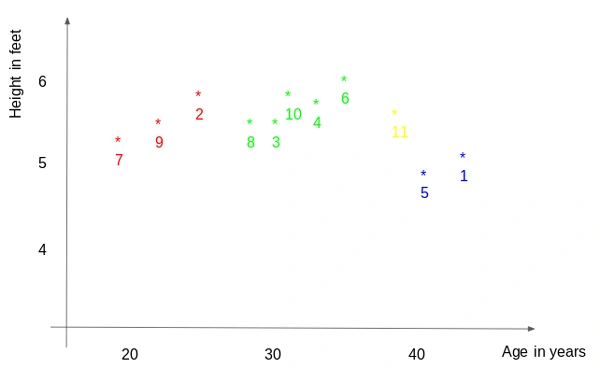
\includegraphics[width=0.7\textwidth]{Img/Screenshot-from-2018-08-22-12-49-19.png}
    \caption{Simple example coordinate graph}
\end{figure}


\begin{figure}[H]
    \centering
    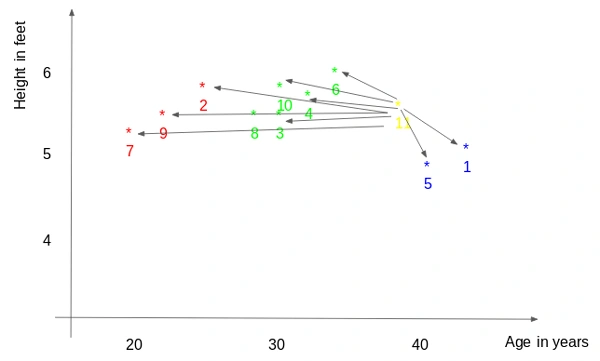
\includegraphics[width=0.7\textwidth]{Img/Screenshot-from-2018-08-22-12-49-33.png}
    \caption{Calculate the distance between the new point and each training point}
\end{figure}

\paragraph{k 值的选择}
k值的选择是 kNNR 算法的关键参数之一。如果 $k$ 值选择过小,模型容易受到噪声的影响,导致过拟合;如果 $k$ 值选择过大,模型会过于平滑,忽略了局部的特征信息,导致欠拟合。通常可以通过交叉验证的方法来选择合适的 $k$ 值,即在训练集上划分不同的验证集,对不同的 $k$ 值进行测试,选择使得验证集上分类准确率最高的 $k$ 值。

\begin{figure}[H]
    \centering
    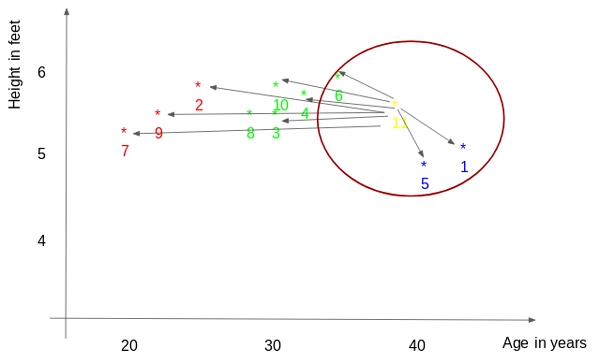
\includegraphics[width=0.7\textwidth]{Img/Screenshot-from-2018-08-22-12-50-04.png}
    \caption{For a value k = 3, the closest points are ID1, ID5, and ID6.}
\end{figure}

\begin{figure}[H]
    \centering
    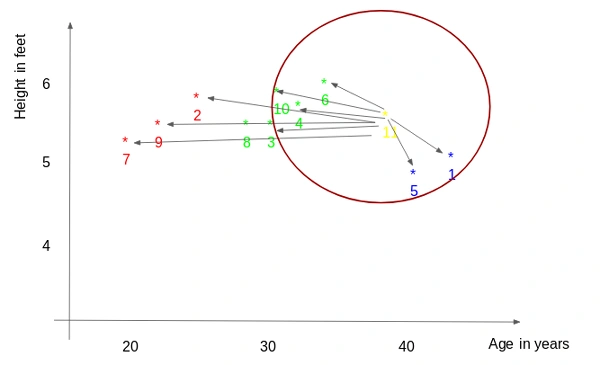
\includegraphics[width=0.7\textwidth]{Img/Screenshot-from-2018-08-22-12-50-16.png}
    \caption{For the value of k = 5, the closest point will be ID1, ID4, ID5, ID6, and ID10.}
\end{figure}

\paragraph{投票决策}
选取距离 $x$ 最近的 $k$ 个样本,这 $k$ 个样本构成一个邻域。统计邻域中各个类别出现的次数,设类别 $c$ 出现的次数为 $n_{c}$。预测待识别样本 $x$ 的类别为出现次数最多的类别,即:
\[
\hat{y}=\arg\max_{c}n_{c}
\]
如果存在多个类别出现次数相同的情况,即有多个 $c$ 使得 $n_{c}$ 最大,则在这些类别对应的样本中,选择距离 $x$ 最近的样本所属的类别作为待识别样本 $x$ 的预测类别。

\paragraph{阈值的作用}
在人脸识别系统中,阈值用于控制识别的严格程度。具体来说,阈值决定了待识别样本与训练样本之间的最小距离。如果待识别样本与最近邻样本的距离小于阈值,则认为识别成功;否则,识别失败,返回“陌生人”结果。阈值的设置直接影响系统的识别准确率和误识别率。较低的阈值会增加系统的灵敏度,但可能导致更多的误识别;较高的阈值会提高系统的准确性,但可能导致漏识别。

\paragraph{阈值的动态调整}
为了适应不同的应用场景和需求,系统提供了动态调整阈值的功能。用户可以通过滑块控件实时调整阈值,观察识别结果的变化,从而找到最适合当前场景的阈值设置。

\subsubsection{kNNR 在人脸识别中的优势}
\begin{itemize}
    \item \textbf{简单易懂}:kNNR 算法的原理简单直观,不需要复杂的模型训练过程,只需要存储训练样本和对应的类别标签即可。在进行预测时,只需要计算待识别样本与训练样本的距离,然后进行投票决策,易于实现和理解。
    \item \textbf{适应性强}:kNNR 算法不需要对数据的分布进行假设,能够适应各种不同类型的数据。在人脸识别中,由于人脸图像的多样性和复杂性,数据的分布往往比较复杂,kNNR算法能够较好地处理这种情况,具有较强的适应性。
    \item \textbf{局部性好}:kNNR 算法是一种基于局部信息的分类算法,它只考虑待识别样本周围的邻居样本,能够捕捉到数据的局部特征。在人脸识别中,局部特征对于区分不同的人脸具有重要的意义,kNNR 算法能够充分利用这些局部特征,提高识别的准确性。
\end{itemize}
\newpage
\section{核心代码及其解释}

\subsection{PCA 核心代码与解释}

\subsubsection{代码片段 1:PCA 数据预处理}
\begin{lstlisting}[basicstyle=\scriptsize\ttfamily, linewidth=\textwidth]
def fit(self, keep_components_ratio):
    # 计算均值脸
    self.mean_face = self.train_matrix.mean(axis=1, keepdims=True)
    # 数据中心化
    self.centered_data = self.train_matrix - self.mean_face

    # 计算协方差矩阵
    cov_matrix = np.dot(self.centered_data.T, self.centered_data) / (self.train_matrix.shape[1] - 1)
    # 特征值分解
    eig_vals, eig_vecs = np.linalg.eig(cov_matrix)
    # 对特征值排序
    sorted_indices = np.argsort(eig_vals)[::-1]
    eig_vecs = eig_vecs[:, sorted_indices]
    eig_vals = eig_vals[sorted_indices]

    # 计算累计方差贡献率
    eig_vals_total = np.sum(eig_vals)
    variance_explained = np.cumsum(eig_vals) / eig_vals_total
    # 选择主成分数量
    num_components = np.argmax(variance_explained >= keep_components_ratio) + 1

    # 选择前 k 个特征向量
    eig_vecs = eig_vecs[:, :num_components]
    # 计算特征脸
    self.eigenfaces = np.dot(self.centered_data, eig_vecs)
    # 归一化特征脸
    eigenface_norms = np.linalg.norm(self.eigenfaces, axis=0, keepdims=True)
    eigenface_norms[eigenface_norms == 0] = 1
    self.eigenfaces /= eigenface_norms
\end{lstlisting}

\subsubsection{代码片段 1 文字解释}
\begin{itemize}
    \item \textbf{均值脸计算}:
    \begin{itemize}
        \item 均值脸是所有人脸图像的平均特征,反映了人脸的基本结构。通过计算均值脸,我们可以将所有人脸图像对齐到一个共同的中心点,便于后续的特征提取。
        \item 代码中,\texttt{self.mean\_face = self.train\_matrix.mean(axis=1, keepdims=True)} 计算了训练数据的均值脸。
        \item \texttt{self.centered\_data = self.train\_matrix - self.mean\_face} 将数据中心化,使得数据分布以原点为中心。
    \end{itemize}
    \item \textbf{协方差矩阵计算}:
    \begin{itemize}
        \item 协方差矩阵反映了数据各个维度之间的相关性。在人脸识别中,协方差矩阵描述了人脸图像各个像素之间的相关性。
        \item 代码中,\texttt{cov\_matrix = np.dot(self.centered\_data.T, self.centered\_data) / (self.train\_matrix.shape[1] - 1)} 计算了中心化数据的协方差矩阵。
    \end{itemize}
    \item \textbf{特征值分解}:
    \begin{itemize}
        \item 特征值分解是 PCA 的核心步骤,通过分解协方差矩阵,我们可以得到特征值和特征向量。特征值表示数据在各个方向上的方差大小,特征向量表示数据的变化方向。
        \item 代码中,\texttt{eig\_vals, eig\_vecs = np.linalg.eig(cov\_matrix)} 对协方差矩阵进行特征值分解。
        \item \texttt{sorted\_indices = np.argsort(eig\_vals)[::-1]} 对特征值从大到小排序。
    \end{itemize}
    \item \textbf{选择主成分}:
    \begin{itemize}
        \item 主成分是数据中最具变化性的方向,选择合适的主成分数量可以在保留足够信息的同时降低数据维度。
        \item 代码中,\texttt{variance\_explained = np.cumsum(eig\_vals) / eig\_vals\_total} 计算了累计方差贡献率。
        \item \texttt{num\_components = np.argmax(variance\_explained >= keep\_components\_ratio) + 1} 根据设定的保留比例(如 95\%)选择主成分数量。
    \end{itemize}
    \item \textbf{特征脸计算}:
    \begin{itemize}
        \item 特征脸是 PCA 提取的关键特征,代表了人脸图像中最具变化性的方向。
        \item 代码中,\texttt{self.eigenfaces = np.dot(self.centered\_data, eig\_vecs)} 将中心化数据投影到特征向量空间,得到特征脸。
    \end{itemize}
\end{itemize}

\subsection{kNN 核心代码与解释}

\subsubsection{代码片段 2:kNN 分类器}
\begin{lstlisting}[basicstyle=\scriptsize\ttfamily, linewidth=\textwidth]
def kNNR_classifier(self, distances, k, train_labels):
    # 找到距离最近的 k 个邻居
    knn_indices = np.argpartition(distances, k - 1)[:k]
    knn_labels = train_labels[knn_indices]

    # 统计 k 个邻居中每个标签出现的次数
    unique_labels, counts = np.unique(knn_labels, return_counts=True)
    max_count = counts.max()
    candidate_labels = unique_labels[counts == max_count]

    # 处理平局情况
    best_index = None
    best_distance = float('inf')
    for label in candidate_labels:
        indices = knn_indices[knn_labels == label]
        local_idx = indices[np.argmin(distances[indices])]
        if distances[local_idx] < best_distance:
            best_distance = distances[local_idx]
            best_index = local_idx

    return best_index
\end{lstlisting}

\subsubsection{代码片段 2 文字解释}
\begin{itemize}
    \item \textbf{选择最近邻}:
    \begin{itemize}
        \item kNN 算法的核心思想是通过计算待识别样本与训练样本的距离,找到距离最近的 k 个邻居。
        \item 代码中,\texttt{knn\_indices = np.argpartition(distances, k - 1)[:k]} 找到距离最近的 k 个邻居的索引。
        \item \texttt{knn\_labels = train\_labels[knn\_indices]} 获取这 k 个邻居的标签。
    \end{itemize}
    \item \textbf{投票决策}:
    \begin{itemize}
        \item 在 k 个邻居中,统计每个标签出现的次数,选择出现次数最多的标签作为预测结果。
        \item 代码中,\texttt{unique\_labels, counts = np.unique(knn\_labels, return\_counts=True)} 统计 k 个邻居中每个标签出现的次数。
        \item \texttt{max\_count = counts.max()} 找到出现次数最多的标签。
    \end{itemize}
    \item \textbf{处理平局}:
    \begin{itemize}
        \item 如果多个标签出现次数相同,选择距离最近的样本的标签作为最终预测结果。
        \item 代码中,\texttt{best\_index = None} 和 \texttt{best\_distance = float('inf')} 用于记录距离最近的样本索引。
    \end{itemize}
\end{itemize}

\subsection{人脸检测核心代码与解释}

\subsubsection{代码片段 3:人脸检测}
\begin{lstlisting}[basicstyle=\scriptsize\ttfamily, linewidth=\textwidth]
def detect_faces(self, image):
    (h, w) = image.shape[:2]
    blob = cv2.dnn.blobFromImage(cv2.resize(image, (300, 300)), 1.0, (300, 300), (104.0, 177.0, 123.0))
    self.net.setInput(blob)
    return self.net.forward()
\end{lstlisting}

\subsubsection{代码片段 3 文字解释}
\begin{itemize}
    \item \textbf{图像预处理}:
    \begin{itemize}
        \item 人脸检测的第一步是将输入图像调整为固定大小(如 300x300),并进行归一化处理。
        \item 代码中,\texttt{blob = cv2.dnn.blobFromImage(...)} 将输入图像调整为 300x300 大小,并进行归一化处理。
    \end{itemize}
    \item \textbf{人脸检测}:
    \begin{itemize}
        \item 使用预训练的深度学习模型进行人脸检测,返回检测结果。
        \item 代码中,\texttt{self.net.setInput(blob)} 将预处理后的图像输入到神经网络中。
        \item \texttt{return self.net.forward()} 返回神经网络的人脸检测结果。
    \end{itemize}
\end{itemize}

\subsection{数据集处理核心代码与解释}

\subsubsection{代码片段 4:数据集分割}
\begin{lstlisting}[basicstyle=\scriptsize\ttfamily, linewidth=\textwidth]
def split_dataset(self, matrix, labels, train_ratio):
    train_data = []
    train_labels = []
    test_data = []
    test_labels = []
    for label in np.unique(labels):
        indices = np.where(labels == label)[0]
        indices = np.random.permutation(indices)
        train_num = int(len(indices) * train_ratio)
        train_indices = indices[:train_num]
        test_indices = indices[train_num:]
        train_data.append(matrix[:, train_indices])
        test_data.append(matrix[:, test_indices])
        train_labels.extend([label] * len(train_indices))
        test_labels.extend([label] * len(test_indices))

    train_data = np.hstack(train_data)
    test_data = np.hstack(test_data)
    train_labels = np.array(train_labels)
    test_labels = np.array(test_labels)
    return train_data, train_labels, test_data, test_labels
\end{lstlisting}

\subsubsection{代码片段 4 文字解释}
\begin{itemize}
    \item \textbf{数据集分割}:
    \begin{itemize}
        \item 按照设定的训练比例(如 80\%)将数据集分为训练集和测试集。
        \item 代码中,\texttt{train\_num = int(len(indices) * train\_ratio)} 计算每个类别的训练样本数量。
        \item \texttt{train\_indices = indices[:train\_num]} 和 \texttt{test\_indices = indices[train\_num:]} 分别获取训练集和测试集的索引。
    \end{itemize}
    \item \textbf{数据合并}:
    \begin{itemize}
        \item 将每个类别的训练数据和测试数据合并为完整的训练集和测试集。
        \item 代码中,\texttt{train\_data = np.hstack(train\_data)} 和 \texttt{test\_data = np.hstack(test\_data)} 将每个类别的数据合并。
    \end{itemize}
\end{itemize}

\subsection{图像预处理核心代码与解释}

\subsubsection{代码片段 5:图像增强}
\begin{lstlisting}[basicstyle=\scriptsize\ttfamily, linewidth=\textwidth]
def enhance_image(self, image, remove_background=True):
    ycrcb_face = cv2.cvtColor(image, cv2.COLOR_BGR2YCR_CB)
    channels = cv2.split(ycrcb_face)
    channels = list(channels)
    clahe = cv2.createCLAHE(clipLimit=2.0, tileGridSize=(8,8))
    channels[0] = clahe.apply(channels[0])
    cv2.merge(channels, ycrcb_face)
    image = cv2.cvtColor(ycrcb_face, cv2.COLOR_YCR_CB2BGR)
    if remove_background:
        blurred_face = cv2.GaussianBlur(image, (7, 7), 0)
        mask = np.zeros(image.shape[:2], np.uint8)
        bgd_model = np.zeros((1, 65), np.float64)
        fgd_model = np.zeros((1, 65), np.float64)
        rect = (int(Config.RECOGNITION_SIZE * 0.04),
                int(Config.RECOGNITION_SIZE * 0.04),
                image.shape[1] - int(Config.RECOGNITION_SIZE * 0.08),
                image.shape[0] - int(Config.RECOGNITION_SIZE * 0.08))
        cv2.grabCut(blurred_face, mask, rect, bgd_model, fgd_model, 1, cv2.GC_INIT_WITH_RECT)
        mask2 = np.where((mask == cv2.GC_FGD) | (mask == cv2.GC_PR_FGD), 1, 0).astype('uint8')
        grabbed_face = image * mask2[:, :, np.newaxis]
        image = cv2.cvtColor(grabbed_face, cv2.COLOR_BGR2GRAY)
    else:
        image = cv2.cvtColor(image, cv2.COLOR_BGR2GRAY)
    return image
\end{lstlisting}

\subsubsection{代码片段 5 文字解释}
\begin{itemize}
    \item \textbf{图像增强}:
    \begin{itemize}
        \item 使用 CLAHE(对比度受限的自适应直方图均衡化)增强图像的对比度,使得人脸特征更加明显。
        \item 代码中,\texttt{clahe = cv2.createCLAHE(clipLimit=2.0, tileGridSize=(8,8))} 创建 CLAHE 对象。
        \item \texttt{channels[0] = clahe.apply(channels[0])} 对图像的亮度通道进行增强。
    \end{itemize}
    \item \textbf{背景去除}:
    \begin{itemize}
        \item 使用 GrabCut 算法去除图像背景,保留人脸区域,减少背景对识别结果的干扰。
        \item 代码中,\texttt{cv2.grabCut(...)} 使用 GrabCut 算法去除背景。
        \item \texttt{mask2 = np.where((mask == cv2.GC\_FGD) | (mask == cv2.GC\_PR\_FGD), 1, 0).astype('uint8')} 生成背景掩码。
        \item \texttt{grabbed\_face = image * mask2[:, :, np.newaxis]} 保留前景区域。
    \end{itemize}
\end{itemize}
\newpage
\section{项目识别结果分析}

\subsection{对于本地数据集测试}

\begin{table}[H]
    \centering
    \begin{tabular}{|c|c|c|c|c|}
        \hline
        数据集 & 测试样本数 & 正确识别数 & 识别率 & 备注 \\
        \hline
        Att\_Faces & 训练 120 张,测试 30 张 & 23 & 76.66\% & 无背景干扰,识别率较高。 \\
        \hline
        Dataset\_Pure & 训练 100 张,测试 25 张 & 18 & 72\% & 无背景干扰,识别率较高。 \\
        \hline
    \end{tabular}
    \caption{本地数据集测试结果}
\end{table}

\subsection{对于调用摄像头测试}

\begin{table}[H]
    \centering
    \begin{tabular}{|c|c|c|}
        \hline
        & With Background & Remove Background \\
        \hline
        条件 & 对于背景要求较严 & 不需要严格纯净的背景 \\
        \hline
        识别率 & 在特定角度下能够稳定识别 & 能够较为快速、准确的识别 \\
        \hline
        截图 & 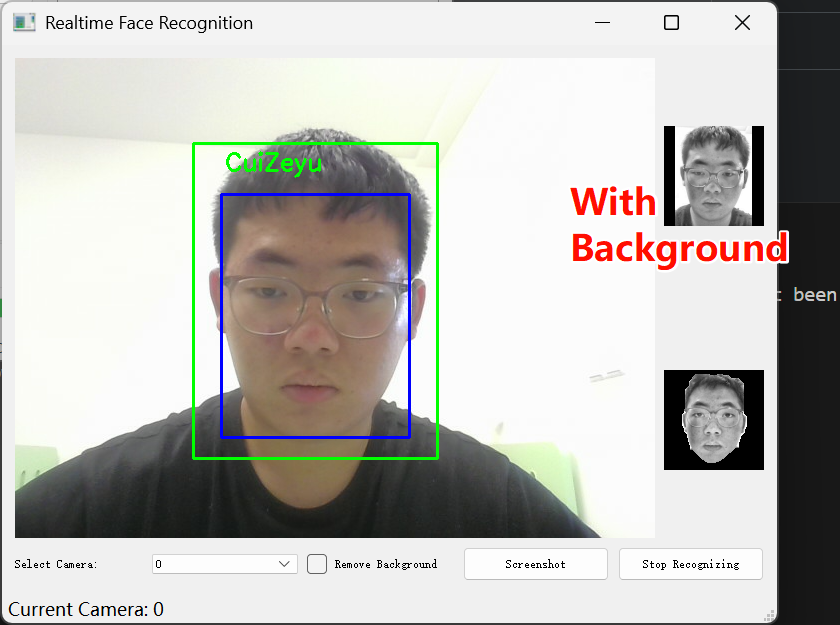
\includegraphics[width=0.4\textwidth]{Img/PixPin_2025-03-09_11-53-03.png} & 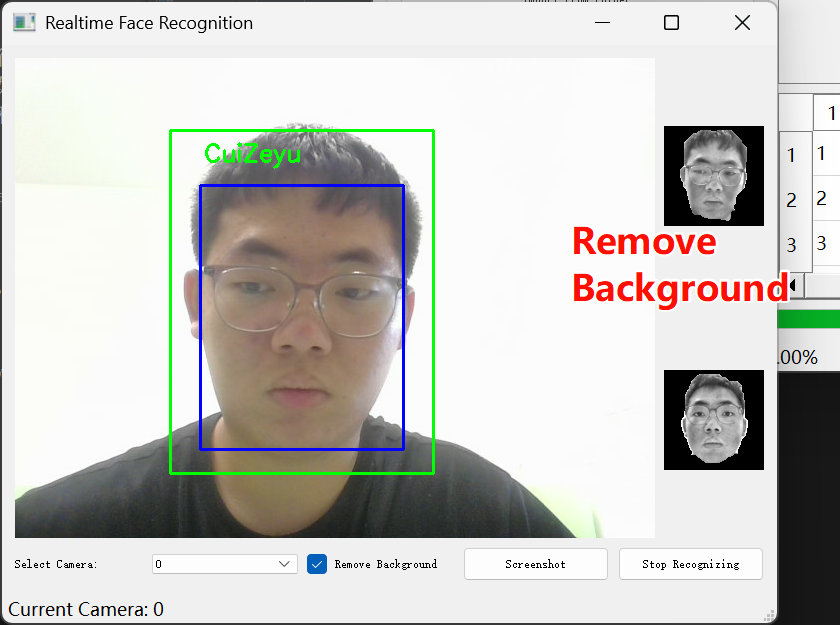
\includegraphics[width=0.4\textwidth]{Img/PixPin_2025-03-09_11-54-41.png} \\
        \hline
    \end{tabular}
    \caption{调用摄像头测试结果}
\end{table}
\newpage
\section{使用场景}

\subsection{安防监控领域}

\subsubsection{公共场所安全保障}
在机场、火车站、地铁站等交通枢纽,人员流动频繁且复杂,利用本基于 PCA 的人脸识别系统能够实时监控人员身份。系统可与监控摄像头相连,对进入场所的人员进行快速识别。一旦发现黑名单人员,系统能立即发出警报,通知安保人员采取相应措施。

\subsubsection{小区与企业安保}
对于住宅小区和企业办公场所,该系统可作为门禁系统的重要组成部分。居民或员工在进入小区或办公区域时,只需通过人脸识别设备进行身份验证,系统即可快速判断是否为授权人员。

\subsubsection{动态调整阈值以适应不同场景}
在安防监控场景中,不同的环境条件(如光照、摄像头角度等)可能会影响人脸识别的准确性。系统提供的阈值调整功能允许安保人员根据实际情况动态调整识别阈值。例如,在光线较暗的环境中,可以适当降低阈值以提高识别的灵敏度;在光线充足的环境中,可以适当提高阈值以减少误识别。

\subsection{金融支付领域}

\subsubsection{刷脸支付}
在移动支付场景中,本系统可用于刷脸支付的身份验证环节。用户在进行支付操作时,只需面对支付设备的摄像头,系统通过识别用户的人脸特征,与预先注册的人脸信息进行比对。

\subsubsection{银行开户与身份验证}
银行在办理开户业务时,可利用该人脸识别系统对客户身份进行核实。通过采集客户的人脸图像,并与身份证上的照片进行比对,确保开户人身份的真实性。同时,在后续的业务操作中,如大额取款、转账等,也可使用人脸识别进行身份验证,进一步保障客户资金安全。

\subsection{教育领域}

\subsubsection{考勤管理}
学校可以使用本系统进行学生考勤管理。在教室门口安装人脸识别设备,学生进入教室时,系统自动识别学生身份并记录考勤信息。这避免了传统考勤方式中代签、漏签等问题,提高了考勤管理的准确性和效率教师可以通过系统随时查看学生的考勤情况,及时掌握学生的出勤状态。

\subsubsection{考试监考}
在考试过程中,利用人脸识别系统对考生身份进行验证,防止替考现象的发生。考生进入考场前,需通过人脸识别设备进行身份确认,系统将现场采集的人脸图像与考生报名时的照片进行比对。
\newpage
\section{项目总结}

\subsection{项目成果总结分析}
本项目成功设计并实现了一个基于 PCA 的人脸识别系统,通过综合运用 PCA 技术进行特征提取和kNNR算法进行分类识别,有效地完成了人脸图像的识别任务。系统在数据处理、特征提取和分类识别等方面展现出了较高的性能和准确性,同时具备良好的用户体验和扩展性。

在数据处理阶段,系统采用了灵活的预处理策略,包括图像裁剪、缩放和背景去除等操作,提高了图像数据的质量。PCA 参数的自动选择机制确保了在保留关键特征的同时,有效降低了数据维度,实现了计算效率和识别精度的平衡。kNNR 算法的简单易懂和适应性强的特点,使得系统能够较好地处理不同类型的人脸数据。

项目提供的阈值调整功能极大地增强了系统的灵活性和适用性。用户可以根据不同的应用场景和需求,动态调整识别阈值,以达到最佳的识别效果。这一功能不仅提高了系统的实用性,还为用户提供了更多的操作自由度,使得系统能够更好地适应复杂多变的实际环境。

通过基于 \texttt{PyQt5} 开发的用户界面,系统实现了高度集成化,用户可以方便地进行数据导入、模型训练、相机操作和数据集管理等操作。系统还提供了数据集保存和加载功能,方便用户对数据进行管理和复用。

\subsection{局限性分析}
尽管本系统取得了一定的成果,但仍存在一些局限性。在复杂环境下,如光照变化剧烈、人脸姿态较大或存在遮挡等情况,系统的识别准确率会受到一定影响。这是因为 PCA 技术主要基于全局特征,对于局部特征的捕捉能力相对较弱。此外,kNNR 算法在处理大规模数据集时,计算复杂度较高,识别速度会有所下降。

\subsection{未来展望}
为了进一步提升系统的性能和适用性,未来可以从以下几个方面进行优化和拓展:

\begin{itemize}
    \item \textbf{引入深度学习技术}:深入研究并尝试使用更复杂、更先进的深度学习模型,如卷积神经网络(CNN)、人脸识别专用网络(如 FaceNet、ArcFace 等)进行特征提取和分类。深度学习模型能够自动学习到更丰富、更具判别性的特征,在复杂环境下具有更好的识别性能。
    \item \textbf{多模态融合}:将人脸识别与其他生物识别技术(如指纹识别、虹膜识别)进行融合,提高系统的安全性和可靠性。多模态识别可以综合利用不同生物特征的优势,减少单一特征识别的局限性。
    \item \textbf{优化算法性能}:针对 kNNR 算法计算复杂度高的问题,研究并采用更高效的算法或数据结构进行优化,如使用 KD 树、球树等加速最近邻搜索过程,提高识别速度。
    \item \textbf{拓展应用场景}:进一步探索系统在更多领域的应用,如智能家居、智能安防、医疗健康等。根据不同应用场景的需求,对系统进行定制化开发,提高系统的通用性和实用性。
\end{itemize}

总体而言,本基于 PCA 的人脸识别系统为后续的研究和开发提供了一个良好的基础,通过不断的优化和拓展,有望在人脸识别领域发挥更大的作用。

\section*{参考内容}
\begin{itemize}
    \item \href{https://en.wikipedia.org/wiki/K-nearest_neighbors_algorithm}{k-nearest neighbors algorithm}
    \item \href{https://en.wikipedia.org/wiki/Principal_component_analysis}{Principal component analysis}
    \item \href{https://zh.wikipedia.org/wiki/%E7%89%B9%E5%BE%81%E8%84%B8}{特征脸}
    \item \href{https://zhuanlan.zhihu.com/p/356640804}{基于 PCA 的人脸识别方法——特征脸法}
    \item \href{https://medium.com/towards-data-science/pca-principal-component-analysis-explained-visually-in-5-minutes-20ce8a9ebf0f}{PCA (Principal Component Analysis) Explained Visually In 5 Minutes}
    \item \href{https://www.analyticsvidhya.com/blog/2018/08/k-nearest-neighbor-introduction-regression-python}{KNN algorithm: Introduction to K-Nearest Neighbors Algorithm for Regression}
\end{itemize}

\end{document}